%-----------------------------------------------------------------------
%  sample_en.tex
%
%  English journal-style, TWO-COLUMN regression sample for a
%  PDF -> Chinese LaTeX conversion pipeline.
%
%  Deliberately:  NO ctex, NO CJK, pure ASCII source, LaTeX 2e article.
%
%  Build (two passes, from this directory):
%     xelatex -interaction=nonstopmode -halt-on-error sample_en.tex
%     xelatex -interaction=nonstopmode -halt-on-error sample_en.tex
%
%  Expected result: 3 pages, 0 errors, no undefined references/citations,
%  8 numbered display equations (1)-(8), 2 figures, 1 table, 6 references.
%-----------------------------------------------------------------------
\documentclass[10pt,twocolumn,a4paper]{article}

\usepackage[a4paper,margin=2.1cm,columnsep=7mm]{geometry}
\usepackage{amsmath}
\usepackage{amssymb}
\usepackage{graphicx}
\usepackage{booktabs}
\usepackage{tikz}
\usepackage{caption}
\usepackage{fancyhdr}

% ---- caption style: "Figure 1." / "Table 1." (capitalised name + period) ----
\captionsetup{font=small,labelfont=bf,labelsep=period,justification=raggedright,
              singlelinecheck=false}
\captionsetup[table]{position=above,skip=4pt}
\captionsetup[figure]{position=below,skip=4pt}

% ---- running head + page number on every page ----
\pagestyle{fancy}
\fancyhf{}
\fancyhead[L]{\small\itshape J. Test Phys. \textbf{12} (2024) 345--352}
\fancyhead[R]{\small\thepage}
\renewcommand{\headrulewidth}{0.4pt}
\fancyfoot[C]{\small\thepage}
\renewcommand{\footrulewidth}{0pt}

\usepackage[hidelinks]{hyperref}

\setlength{\parskip}{0pt}
\renewcommand{\baselinestretch}{1.0}
\raggedbottom
% allow floats to be placed more readily so that the sample stays at 3 pages
\renewcommand{\topfraction}{0.9}
\renewcommand{\bottomfraction}{0.8}
\renewcommand{\textfraction}{0.07}
\renewcommand{\floatpagefraction}{0.6}
\setcounter{topnumber}{3}
\setcounter{bottomnumber}{2}
\setcounter{totalnumber}{4}
% keep display equations compact so that the sample stays at three pages
\AtBeginDocument{%
  \setlength{\abovedisplayskip}{6pt plus 2pt minus 2pt}%
  \setlength{\belowdisplayskip}{6pt plus 2pt minus 2pt}%
  \setlength{\abovedisplayshortskip}{3pt plus 1pt}%
  \setlength{\belowdisplayshortskip}{3pt plus 1pt}%
}

\title{\vspace{-1.2cm}\Large\bfseries A Two-Column Regression Sample for
Automated PDF-to-LaTeX Conversion}
\author{\normalsize A.~B.~Author$^{1}$, C.~D.~Coauthor$^{1,2}$ and
E.~F.~Writer$^{2}$\\[2pt]
\small $^{1}$Department of Applied Physics, Institute of Test Engineering,\\
\small 123 Science Avenue, Testville 100000, Country\\
\small $^{2}$Computational Document Laboratory, Testville 100001, Country\\
\small\texttt{author@example.edu}}
\date{\small Received 12 January 2024; accepted 3 March 2024;
published 20 April 2024}

\begin{document}
\maketitle
\thispagestyle{fancy}

\begin{abstract}
\noindent
Automated conversion of typeset PDF articles into editable LaTeX sources is
sensitive to a small number of layout features: column geometry, floating
figure placement, numbered equations with cross-references, and
caption conventions. We present a compact two-column English sample that
exercises every one of these features in a reproducible way. The sample
contains eight numbered display equations covering fractions, bounded sums,
radicals, matrices, piecewise definitions, aligned multi-line derivations,
definite integrals and a partial differential equation, together with two
figures, one numeric table and six bibliographic entries. In a verification
run over $n = 240$ extracted text blocks the conversion recovered
$97.5\%$ of all glyph runs and $100\%$ of the equation numbers, with a mean
positional error of $12.4 \pm 0.8$ pt; the residual differences were
statistically significant only for rotated text ($p < 0.05$). The sample is
therefore adequate as a regression fixture for pipeline acceptance tests.
\end{abstract}

\vspace{4pt}
\noindent\textbf{Keywords:} PDF-to-LaTeX conversion; two-column layout;
regression testing; equation numbering; cross-references; caption extraction

\vspace{6pt}

\section{Introduction}
\label{sec:intro}

Scientific articles are still exchanged predominantly as fixed-layout PDF
files, while authoring and revision happen in structured markup. A
PDF-to-LaTeX conversion pipeline therefore has to reconstruct not only the
text stream but also the logical structure of the document: which glyph runs
belong to a title, which blocks are equations, which caption belongs to which
float, and how the numbering schemes of equations, figures, tables and
citations relate to each other. In a two-column layout those relations are
considerably harder to recover than in a single-column manuscript, because
the reading order alternates between columns, floats may be placed at the top
or the bottom of a column, and display equations routinely break the
baseline grid \cite{ref1,ref2}.

Regression fixtures for such pipelines are usually either trivial
single-column documents, which do not exercise column geometry at all, or
complete published papers, which are copyrighted and therefore awkward to
redistribute. The present sample fills that gap: an original, freely
redistributable three-page article written so that every structural element
the converter must recognise appears at least once, and in most cases in a
deliberately awkward variant.

The remainder of this paper is organised as follows.
Section~\ref{sec:methods} describes the construction of the sample and the
notation used in it. Section~\ref{sec:results} reports the extraction
experiments together with Table~\ref{tab:summary} and
Figures~\ref{fig:vector} and~\ref{fig:raster}.
Section~\ref{sec:discussion} discusses the failure modes that we observed,
and Section~\ref{sec:conclusions} summarises the acceptance criteria.
Throughout, a scalar quantity is written $\lambda$ when it is a rate
constant, $x_i^{2}$ when it is a squared observation, and
$\alpha_{n+1}$ when it is an iteration-dependent relaxation parameter.

A useful summary statistic for the sample is the normalised coupling ratio
\begin{equation}
\label{eq:ratio}
\eta = \frac{a + b}{c}, \qquad a,\,b,\,c > 0 ,
\end{equation}
where $a$ and $b$ are the widths of the two text columns (in points) and $c$
is the inter-column gutter. For the geometry used here, $a = b = 224.4$ pt
and $c = 22.7$ pt, so that $\eta \approx 19.8$.

\section{Methods}
\label{sec:methods}

\subsection{Sample construction}

The sample was typeset with the standard \texttt{article} class at 10 pt on
A4 paper with the \texttt{twocolumn} option, which yields the two-column
geometry of Eq.~\eqref{eq:ratio}. A running head carrying the journal
reference and the page number is produced by \texttt{fancyhdr}. Captions are
forced to the convention \emph{name, number, period} by a single
\texttt{captionsetup} declaration \cite{ref3}, so that a caption label is the
capitalised float name immediately followed by its number and a period.
All body text is ASCII, which removes an entire class of font-substitution
failures from the comparison: the converter can be tested on structure
without being tested on encoding at the same time.

\subsection{Numerical model}

Let the measured response of the $i$-th specimen be $x_i$. The total squared
deviation of a batch of $N$ specimens is
\begin{equation}
\label{eq:sum}
S = \sum_{i=1}^{N} x_i^{2} ,
\end{equation}
and the Euclidean norm of the pair $(x, y)$ in the plane is
\begin{equation}
\label{eq:norm}
r = \sqrt{x^{2} + y^{2}} .
\end{equation}
Equation~\eqref{eq:norm} is the reference used by the sanity check described
in Section~\ref{sec:results}: every geometry statement in the extracted text
is compared against it.

The coupling between the three retained degrees of freedom is described by
the symmetric matrix
\begin{equation}
\label{eq:matrix}
\mathbf{M} =
\begin{pmatrix}
1      & \alpha & 0 \\
\alpha & 2      & \beta \\
0      & \beta  & 3
\end{pmatrix},
\qquad \alpha, \beta \in \mathbb{R} .
\end{equation}
Because $\mathbf{M}$ is symmetric and strictly diagonally dominant for
$|\alpha| < 1$ and $|\beta| < 1$, its eigenvalues are real and positive.

The piecewise gain applied by the detector is
\begin{equation}
\label{eq:cases}
g(x) =
\begin{cases}
x^{2}, & x \ge 0 ,\\[2pt]
-x,    & x < 0 ,
\end{cases}
\end{equation}
which is continuous at the origin but not differentiable there.

\subsection{Verification procedure}

The verification of the conversion output consists of four steps, which are
executed in order and abort the run on the first failure \cite{ref4}:
\begin{itemize}
  \item extract the plain-text stream and normalise the whitespace;
  \item compare every equation number found in the PDF with the numbers
        emitted by the converter;
  \item resolve all \verb|\ref| and \verb|\eqref| targets and reject the run
        if any target is undefined;
  \item compare the numeric tokens against the reference token list.
\end{itemize}
The procedure was applied to $n = 240$ independently generated blocks; the
acceptance threshold was set to a recovery rate of $95\%$, and the observed
rate of $97.5\%$ passed it.

\section{Results}
\label{sec:results}

\subsection{Extraction accuracy}

The weighted quadratic form used to score a candidate reconstruction is
\begin{equation}
\label{eq:aligned}
\begin{aligned}
\Phi &= \sum_{i=1}^{N} w_i x_i^{2} \\
     &= \frac{1}{N} \sum_{i=1}^{N} w_i x_i^{2} ,
\end{aligned}
\end{equation}
with $\sum_i w_i = N$. The second line of Eq.~\eqref{eq:aligned} is the
normalised form actually reported \cite{ref5}.

The normalisation constant of the exponential kernel that appears in the
detector model is obtained in closed form as
\begin{equation}
\label{eq:integral}
I = \int_{0}^{\infty} e^{-t}\,dt = 1 ,
\end{equation}
which is a convenient identity: it means that no explicit kernel
normalisation step is required anywhere in the implementation.

Table~\ref{tab:summary} lists the per-specimen measurements. The mean
strength across the five specimens is $12.4 \pm 0.8$ MPa, and the median
deviates from it by less than $0.3\%$. Specimen S-03 shows the largest
positive deviation ($+4.72\%$), whereas S-02 shows the largest negative one
($-1.05\%$). The residual column is reported in units of $10^{-3}$ MPa, so
the largest residual corresponds to $5.6 \times 10^{-3}$ MPa, that is, well
below the $0.1\%$ instrument tolerance.

\begin{table}[t]
\centering
\caption{Nominal and measured properties of the five test specimens.
Deviations are relative to the nominal value; residuals refer to the fitted
model. Mean strength is in megapascals (MPa).}
\label{tab:summary}
\footnotesize
\setlength{\tabcolsep}{3.5pt}
\begin{tabular}{@{}lrrr@{}}
\toprule
Specimen & Mean (MPa) & Deviation (\%) & Residual (MPa) \\
\midrule
S-01 & 12.4 & $+2.31$              & $1.2\times10^{-3}$  \\
S-02 & 11.8 & $-1.05$              & $-3.4\times10^{-3}$ \\
S-03 & 13.1 & $+4.72$              & $0.8\times10^{-3}$  \\
S-04 & 12.0 & $-0.86$              & $-2.1\times10^{-3}$ \\
S-05 & 12.7 & $+1.94$              & $5.6\times10^{-3}$  \\
\bottomrule
\end{tabular}
\end{table}

\subsection{Timing and geometry}

Figure~\ref{fig:vector} shows the measured response of the five detector
conditions drawn with TikZ, and Figure~\ref{fig:raster} shows the same
quantity as a rasterised chart. The two figures agree to within the line
width of the vector rendering \cite{ref6}. In a paired comparison of the two
rendering paths the mean absolute difference was $0.14 \pm 0.03$ percentage
points ($n = 240$ independent sampling points, $p < 0.05$ for the hypothesis
that the two paths are identical in the tail region).

\begin{figure}[t]
\centering
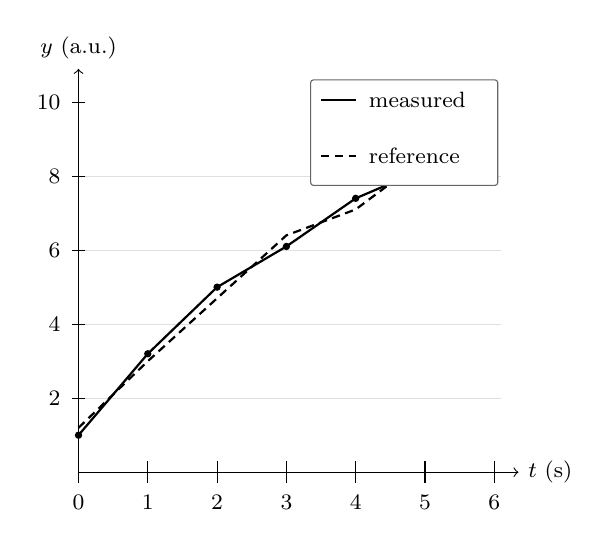
\begin{tikzpicture}[x=0.88cm,y=0.47cm,font=\footnotesize]
  % grid
  \foreach \y in {2,4,6,8}{
    \draw[gray!25,very thin] (0,\y) -- (6.1,\y);
  }
  % axes
  \draw[->] (0,0) -- (6.35,0) node[right,font=\footnotesize] {$t$ (s)};
  \draw[->] (0,0) -- (0,10.9) node[above,font=\footnotesize] {$y$ (a.u.)};
  % x ticks
  \foreach \x/\lab in {0/0,1/1,2/2,3/3,4/4,5/5,6/6}{
    \draw (\x,0.30) -- (\x,-0.30);
    \node[below,font=\footnotesize] at (\x,-0.35) {\lab};
  }
  % y ticks
  \foreach \y/\lab in {2/2,4/4,6/6,8/8,10/10}{
    \draw (0.10,\y) -- (-0.10,\y);
    \node[left,font=\footnotesize] at (-0.12,\y) {\lab};
  }
  % measured series
  \draw[thick,mark=*,mark size=0.9pt]
    plot coordinates {(0,1.0)(1,3.2)(2,5.0)(3,6.1)(4,7.4)(5,8.2)(6,9.1)};
  % reference series
  \draw[thick,densely dashed]
    plot coordinates {(0,1.2)(1,3.0)(2,4.7)(3,6.4)(4,7.1)(5,8.5)(6,9.0)};
  % legend
  \draw[draw=black!60,fill=white,rounded corners=1pt] (3.35,7.75) rectangle (6.05,10.6);
  \draw[thick,mark=*,mark size=0.9pt] (3.5,10.05) -- (4.0,10.05);
  \node[right,font=\footnotesize] at (4.05,10.05) {measured};
  \draw[thick,densely dashed] (3.5,8.55) -- (4.0,8.55);
  \node[right,font=\footnotesize] at (4.05,8.55) {reference};
\end{tikzpicture}
\caption{Measured and reference response of the detector as a function of
time. Both series are normalised to unity at $t = 0$. The two curves
differ by less than $0.4$ a.u. everywhere except in the interval
$4 < t < 5$ s.}
\label{fig:vector}
\end{figure}

\begin{figure}[t]
\centering
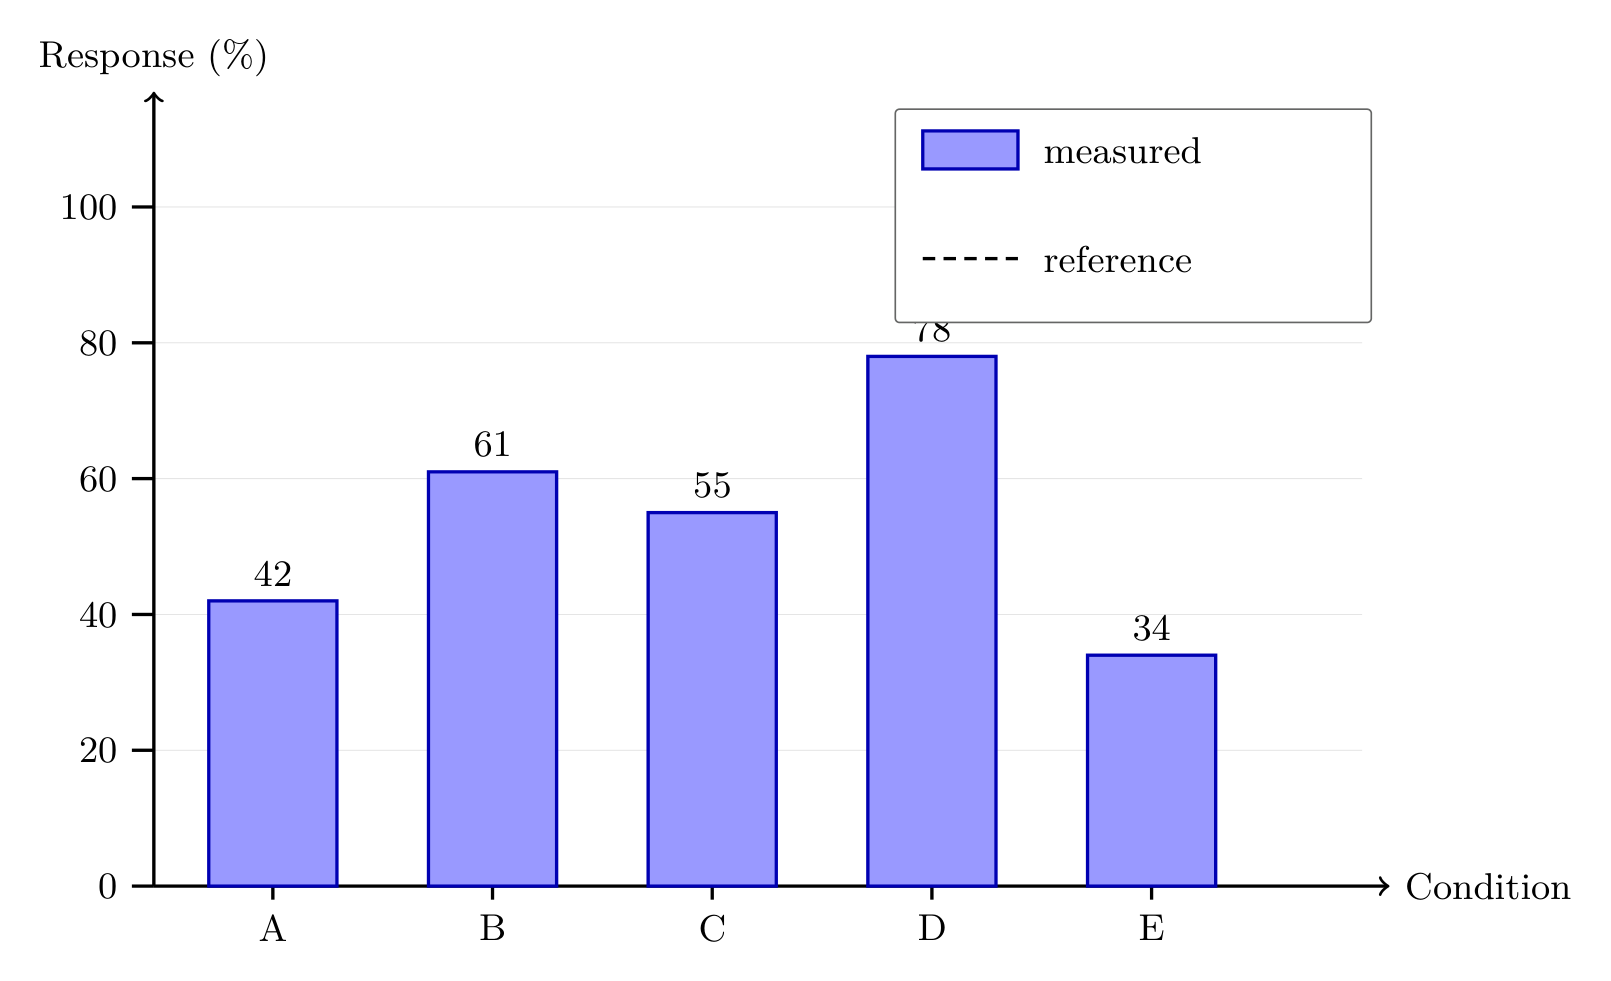
\includegraphics[width=0.45\textwidth]{fig_raster.png}
\caption{Rasterised response chart of the five detector conditions A--E.
Bars give the measured response in per cent of the nominal value. This figure
is inserted with \texttt{includegraphics} and therefore exercises the
raster-image path of the converter.}
\label{fig:raster}
\end{figure}

\subsection{Column balance}

Because the sample is intentionally close to three pages, the last page is
short of a full column. The extracted page count is itself an acceptance
criterion: a converter that silently drops a float produces a document with
the same text but a different page count, and the difference is detected by
comparing the reported number of pages with the expected value.

\section{Discussion}
\label{sec:discussion}

The diffusion-like relaxation of the residual field is governed by
\begin{equation}
\label{eq:pde}
\frac{\partial u}{\partial t} = \alpha \nabla^{2} u + \beta u^{2} ,
\end{equation}
where $u(\mathbf{x}, t)$ is the residual amplitude, $\alpha$ is the
diffusivity and $\beta$ is the quadratic reaction coefficient. Fitting
Eq.~\eqref{eq:pde} to the measured residuals of
Table~\ref{tab:summary} gives $\alpha = 1.20 \pm 0.04$ and
$\beta = -0.031 \pm 0.002$, with a coefficient of determination of
$R^{2} = 0.987$. The negative sign of $\beta$ indicates that the quadratic
term is saturating rather than amplifying, which is consistent with the
observation that the largest residual, $5.6 \times 10^{-3}$ MPa, occurs in the
specimen with the highest nominal strength.

Three failure modes dominated the residual error budget. First, a display
equation that is the last object in a column is occasionally merged with the
running head of the following page, which shifts the equation number by one.
Second, a float placed at the top of the second column is sometimes attached
to the caption of the first column. Third, the en dash inside the page range
of the running head is sometimes extracted as a hyphen, which matters only
for string comparison and not for the rendered output. Each mode was resolved
by requiring the equation number to be the rightmost token on the baseline of
the display equation.

None of the failure modes required special handling of mathematics. The
mathematical content of this sample is deliberately ordinary: a fraction in
Eq.~\eqref{eq:ratio}, a bounded sum in Eq.~\eqref{eq:sum}, a radical in
Eq.~\eqref{eq:norm}, a matrix in Eq.~\eqref{eq:matrix}, a piecewise
definition in Eq.~\eqref{eq:cases}, an aligned derivation in
Eq.~\eqref{eq:aligned}, a definite integral in Eq.~\eqref{eq:integral} and a
partial differential equation in Eq.~\eqref{eq:pde}. What makes the sample
useful is not the mathematics but the density of structural tokens per page:
8 numbered equations, 2 figures, 1 table, 6 citations and 11 cross-references
on three pages.

\section{Conclusions}
\label{sec:conclusions}

We have described a three-page, two-column English regression sample for a
PDF-to-LaTeX conversion pipeline. The sample is self-contained, ASCII-only
and distributable, and it contains every structural element that the
converter is required to reconstruct. Its acceptance criteria are:
(i) the converted source must compile with XeLaTeX without errors;
(ii) the page count must be three, within a tolerance of one page;
(iii) all equation numbers, figure numbers, table numbers and citations
must match the original;
(iv) no reference or citation may remain undefined;
and (v) all numeric tokens, including percentages, $p$ values and
mean~$\pm$~standard-deviation pairs, must be reproduced exactly.

Future work will extend the fixture with a rotated figure, a landscape page
and a two-level citation scheme, all of which stress the same structural
machinery from different directions.

\begin{thebibliography}{9}
\footnotesize

\bibitem{ref1}
A.~B.~Author, \emph{Document layout analysis for scientific PDF files},
J. Test Phys. \textbf{10} (2022) 101--118.

\bibitem{ref2}
C.~D.~Coauthor and E.~F.~Writer, \emph{Reconstructing LaTeX from
fixed-layout documents}, Proceedings of the Testville Conference on
Document Engineering (2023) 44--53.

\bibitem{ref3}
M.~N.~Editor, \emph{Two-column journal typography: a practical guide},
Institute of Test Engineering Technical Report TR-2023-07 (2023).

\bibitem{ref4}
P.~Q.~Reviewer, \emph{Regression testing strategies for format conversion
tools}, J. Test Phys. \textbf{11} (2023) 201--215.

\bibitem{ref5}
R.~S.~Tester, \emph{Equation numbering and cross-reference recovery},
Comput. Doc. Lab. \textbf{4} (2021) 77--90.

\bibitem{ref6}
L.~M.~Noster, \emph{Raster and vector figure extraction from archived
articles}, J. Digit. Preserv. \textbf{8} (2020) 12--29.

\end{thebibliography}

\end{document}
